% Options for packages loaded elsewhere
\PassOptionsToPackage{unicode}{hyperref}
\PassOptionsToPackage{hyphens}{url}
%
\documentclass[
]{article}
\usepackage{amsmath,amssymb}
\usepackage{lmodern}
\usepackage{ifxetex,ifluatex}
\ifnum 0\ifxetex 1\fi\ifluatex 1\fi=0 % if pdftex
  \usepackage[T1]{fontenc}
  \usepackage[utf8]{inputenc}
  \usepackage{textcomp} % provide euro and other symbols
\else % if luatex or xetex
  \usepackage{unicode-math}
  \defaultfontfeatures{Scale=MatchLowercase}
  \defaultfontfeatures[\rmfamily]{Ligatures=TeX,Scale=1}
\fi
% Use upquote if available, for straight quotes in verbatim environments
\IfFileExists{upquote.sty}{\usepackage{upquote}}{}
\IfFileExists{microtype.sty}{% use microtype if available
  \usepackage[]{microtype}
  \UseMicrotypeSet[protrusion]{basicmath} % disable protrusion for tt fonts
}{}
\makeatletter
\@ifundefined{KOMAClassName}{% if non-KOMA class
  \IfFileExists{parskip.sty}{%
    \usepackage{parskip}
  }{% else
    \setlength{\parindent}{0pt}
    \setlength{\parskip}{6pt plus 2pt minus 1pt}}
}{% if KOMA class
  \KOMAoptions{parskip=half}}
\makeatother
\usepackage{xcolor}
\IfFileExists{xurl.sty}{\usepackage{xurl}}{} % add URL line breaks if available
\IfFileExists{bookmark.sty}{\usepackage{bookmark}}{\usepackage{hyperref}}
\hypersetup{
  hidelinks,
  pdfcreator={LaTeX via pandoc}}
\urlstyle{same} % disable monospaced font for URLs
\usepackage[margin=1.0in]{geometry}
\usepackage{longtable,booktabs,array}
\usepackage{calc} % for calculating minipage widths
% Correct order of tables after \paragraph or \subparagraph
\usepackage{etoolbox}
\makeatletter
\patchcmd\longtable{\par}{\if@noskipsec\mbox{}\fi\par}{}{}
\makeatother
% Allow footnotes in longtable head/foot
\IfFileExists{footnotehyper.sty}{\usepackage{footnotehyper}}{\usepackage{footnote}}
\makesavenoteenv{longtable}
\usepackage{graphicx}
\makeatletter
\def\maxwidth{\ifdim\Gin@nat@width>\linewidth\linewidth\else\Gin@nat@width\fi}
\def\maxheight{\ifdim\Gin@nat@height>\textheight\textheight\else\Gin@nat@height\fi}
\makeatother
% Scale images if necessary, so that they will not overflow the page
% margins by default, and it is still possible to overwrite the defaults
% using explicit options in \includegraphics[width, height, ...]{}
\setkeys{Gin}{width=\maxwidth,height=\maxheight,keepaspectratio}
% Set default figure placement to htbp
\makeatletter
\def\fps@figure{htbp}
\makeatother
\setlength{\emergencystretch}{3em} % prevent overfull lines
\providecommand{\tightlist}{%
  \setlength{\itemsep}{0pt}\setlength{\parskip}{0pt}}
\setcounter{secnumdepth}{-\maxdimen} % remove section numbering
\usepackage{helvet}
\renewcommand*\familydefault{\sfdefault}
\usepackage{setspace}
\doublespacing
\usepackage[left]{lineno}
\linenumbers
\usepackage{multirow}
\usepackage{booktabs}
\usepackage{longtable}
\usepackage{array}
\usepackage{multirow}
\usepackage{wrapfig}
\usepackage{float}
\usepackage{colortbl}
\usepackage{pdflscape}
\usepackage{tabu}
\usepackage{threeparttable}
\usepackage{threeparttablex}
\usepackage[normalem]{ulem}
\usepackage{makecell}
\usepackage{xcolor}
\ifluatex
  \usepackage{selnolig}  % disable illegal ligatures
\fi
\newlength{\cslhangindent}
\setlength{\cslhangindent}{1.5em}
\newlength{\csllabelwidth}
\setlength{\csllabelwidth}{3em}
\newenvironment{CSLReferences}[2] % #1 hanging-ident, #2 entry spacing
 {% don't indent paragraphs
  \setlength{\parindent}{0pt}
  % turn on hanging indent if param 1 is 1
  \ifodd #1 \everypar{\setlength{\hangindent}{\cslhangindent}}\ignorespaces\fi
  % set entry spacing
  \ifnum #2 > 0
  \setlength{\parskip}{#2\baselineskip}
  \fi
 }%
 {}
\usepackage{calc}
\newcommand{\CSLBlock}[1]{#1\hfill\break}
\newcommand{\CSLLeftMargin}[1]{\parbox[t]{\csllabelwidth}{#1}}
\newcommand{\CSLRightInline}[1]{\parbox[t]{\linewidth - \csllabelwidth}{#1}\break}
\newcommand{\CSLIndent}[1]{\hspace{\cslhangindent}#1}

\author{}
\date{\vspace{-2.5em}}

\begin{document}

\hypertarget{taxonomic-resolution-matters-for-microbiome-based-classification-of-colorectal-cancer}{%
\section{Taxonomic Resolution Matters for Microbiome-Based
Classification of Colorectal
Cancer}\label{taxonomic-resolution-matters-for-microbiome-based-classification-of-colorectal-cancer}}

\vspace{10mm}

Courtney R. Armour, Begüm D.Topçuoğlu, Andrea Garretto, Patrick D.
Schloss \({^\dagger}\)

\vspace{20mm}

\({\dagger}\) To whom correspondence should be addressed:

\href{mailto:pschloss@umich.edu}{pschloss@umich.edu}

Department of Microbiology

University of Michigan

Ann Arbor, MI 48109

\vspace{20mm}

\textbf{observation format - max 1200 words, 2 figures, 25 ref}

\newpage

\hypertarget{abstract-max-250-words}{%
\subsection{Abstract (max 250 words)}\label{abstract-max-250-words}}

\hypertarget{importance-max-150-words}{%
\subsection{Importance (max 150 words)}\label{importance-max-150-words}}

\newpage

Colorectal cancer is one of the most common cancers in men and women and
a leading cause of cancer related deaths in the United States
(\protect\hyperlink{ref-siegel2020}{1}). Early detection and treatment
are essential to increase survival rates, but for a variety of reasons
including the invasiveness and high cost of screening
(i.e.~colonoscopy), many people do not comply with recommended screening
guidelines (\protect\hyperlink{ref-garcuxeda2011a}{2}) prompting a need
for low cost, non-invasive detection methods. A growing body of research
points to the gut microbiome as a promising target for non-invasive
screening to detect screen relevant neoplasias (neoplasms?) (SRNs)
consisting of pre-cancerous polyps (i.e.~advanced adenomas) and
carcinomas. Efforts to realize the diagnostic potential of the gut
microbiome in detecting SRNs have focused on machine learning (ML)
methods using abundances from operational taxonomic unit (OTU)
classifications based on amplicon sequencing of the 16S rRNA gene \{\}.
However, whether this is the optimal taxonomic resolution for
classifying SRNs from microbiome data is unknown. Additionally, recent
work has pushed for the use of amplicon sequence variants (ASVs) to
replace OTUs for marker-gene analysis because of the improved resolution
with ASVs (\protect\hyperlink{ref-callahan2017}{3}). However, whether
the additional resolution provided by ASVs is useful for ML
classification is unclear \{\}. Since ML classification relies on
consistent differences between groups, its possible that the resolution
at the ASV level is too individualized to accurately differentiate
groups. Topçuoğlu \emph{et al}
(\protect\hyperlink{ref-topuxe7uolu2020}{4}) recently demonstrated
effective application of machine learning (ML) to microbiome based
classification problems and developed a framework for applying ML
practices in a more reproducible way (mikropml). This analysis utilizes
the reproducible framework developed by Topçuoğlu \emph{et al} to
quantify which ML method and taxonomic level produce the best performing
classifier for detecting SRNs from microbiome data.

Utilizing publicly available 16S rRNA sequence data from stool of
patients with SRNs and healthy controls, we generated abundance tables
with Mothur \{\} annotated to Phylum, Class, Order, Family, Genus, OTU
and ASV levels. Using the taxonomic abundance data, we quantified how
accurately samples could be classified as ``normal'' or ``SRN''
(i.e.~advanced adenoma or carcinoma) using five machine learning methods
with the Mikropml R package (methods). Across the five machine learning
methods tested, model performance tended to increase with taxonomic
level usually peaking around genus/OTU level before dropping off
slightly with ASVs (Supplemental Figure 1). Random forest (RF) was
consistently the top performer at most taxonomic levels. Within the RF
model, the highest AUROCs were observed for family (median AUROC:
0.687), genus (median AUROC: 0.686), and OTU (median AUROC: 0.698) level
data with no significant difference between the three (Figure 1A,
Supplemental Figure 2). Performance with ASVs (median AUROC: 0.676) was
significantly lower than OTUs (p \textless{} 0.01), but borderline
equivalent to family (p = 0.06) and genus (p = 0.05) levels (Figure 1A).
These results were consistent for ASVs generated with DADA2
(\protect\hyperlink{ref-callahan2016}{5}) (median AUROC: 0.66). These
results suggest that finer taxonomic resolution is not necessarily
better for identifying individuals with SRNs based on microbiome
composition.

While comparing AUROC values between models is a useful way to assess
the overall model performance, they summarize the performance across all
thresholds and can be misleading since models with the same AUC can have
different ROC curve shapes (\protect\hyperlink{ref-lobo2008}{6}).
Depending on the intended implementation of the model, one may want to
optimize the true-positive rate (or sensitivity) over the false-positive
rate (or 1-specificity), or vice versa. In this case, the optimal model
will detect as many true positives (people with SRNs) as possible. To
further compare the model performance across taxonomic levels we
compared the sensitivity of the models at a specificity of 90\%. The
highest sensitivity values were observed for Family, Genus, and OTU
level data (Figure 1B), consistent with the AUROC results. Phylum,
Class, Order, and ASV sensitivity values were all significantly lower
than Family, Genus, and OTU sensitivity values (Figure 1B). This
analysis further supports that finer resolution is does not improve SRN
detection.

One hypothesis for the observation that model performance increases from
phylum to OTU level then drops slightly at ASV level is that at higher
taxonomic levels (e.g.~phylum) there are too few taxa and too much
overlap to reliably differentiate between cases and controls. At the
level of genus/OTU data there is enough data and variation but at the
ASV level, the data is too specific to individuals and doesn't overlap
enough. Examination of the prevalence of taxa in samples at each level
supports this idea. A majority of taxa are present in greater than 75\%
of samples at the phylum (67\% of taxa) and class (63\% of taxa) levels.
The opposite is observed at the OTU and ASV level where 60\% and 53\% of
taxa respectively are only present in less than 25\% of samples
(Supplemental Figure 3). Of note, the ML pipeline includes a
pre-processing step that occurs prior to training and classifying the ML
models (methods). As part of this step, features are removed that will
not provide useful information to build the model. For example,
perfectly correlated features provide the same information to build the
model and thus can be collapsed. Additionally, features with zero or
near-zero variance will not help the model differentiate groups and thus
can be removed. Interestingly, despite starting with 104106 features at
the ASV level, only 478 (0.5\%) remained after pre-processing. At the
OTU level, 20079 of the 705 features (3.5\%) remained after
preprocessing (Table 1). While the resolution provided by ASVs is useful
in certain contexts \{\}, these results suggest that the resolution is
too fine for use in machine learning classification of SRNs based on
microbiome composition.

A look into the most important taxa at each level for classifying
samples reveals some nesting where several genera and their higher
taxonomic classifications are in the top 10 most important taxa
(Supplemental Figure 4). For example, the genus \emph{Gemella} is an
important taxa at the genus and OTU levels and its higher
classifications are also important (\emph{Firmicutes} \textgreater{}
\emph{Bacilli} \textgreater{} \emph{Bacillales} \textgreater{}
\emph{Bacillales Incertae Sedis XI} \textgreater{} \emph{Gemella}).
\emph{Fusobacterium} displays a similar pattern, except that the family
level classification (\emph{Fusobacteriaceae}) importance is ranked 16th
out of 54 families, a little beyond the top 10. In the case of
unclassified \emph{Lachnospiraceae}, there are several OTUs with this
label that are in the top 10, however at the Genus level this taxon is
ranked lower in importance (21st out of 115 genera) suggesting there may
be some benefit to separating different taxonomic groupings within
\emph{Lachnospiraceae}.

These results demonstrate that consideration of the appropriate
taxonomic resolution for utilizing the microbiome as a predictive tool
is warranted. In general, we found that finer taxonomic resolution
(e.g.~OTU and ASV) does not add additional sensitivity to predicting
SRNs based on microbiome composition. Additionally, at the ASV level the
fine resolution actually impedes model performance due to the sparsity
of shared taxa and leads to decreased model performance. The tendancy
for ASV level annotation to split single bacterial genomes into multiple
taxa \{Pat mSphere 2021\} could also be a contributing factor to the
sparsity of shared taxa. Overall, either Family, Genus, or OTU level
taxonomy appear to perform equally for predicting subjects with SRNs
based on the composition of the gut microbiome. A potential benefit of
utilizing genus or family level data could be that it may allow for
merging data generated from different 16S regions or sequencing
platforms.

\hypertarget{materials-and-methods}{%
\subsection{Materials and Methods}\label{materials-and-methods}}

\textbf{\emph{Dataset.}} Raw 16S rRNA gene amplicon sequence data
isolated from human gut samples \{Baxter\} was downloaded from NCBI SRA
(accession \#). This dataset contains stool samples from 490 subjects.
Based on the available metadata, samples categorized as normal, high
risk normal, or adenoma were labeled ``normal'' for this analysis and
samples categorized as advanced adenoma or carcinoma were labeled as
``screen relevant neoplasia'' (SRN). This resulted in a total of 261
``normal'' samples and 229 ``SRN'' samples.

\textbf{\emph{Data processing.}} Sequence data was processed with Mothur
(1.44.3) using the SILVA reference database (v132) to produce count
tables for phylum, class, order, family, genus, OTU, and ASV following
the Schloss Lab MiSeq SOP described on the Mothur website \{\}. ASV
level data was also produced using DADA2 to ensure consistent results
with a different pipeline. Data was processed following the DADA2
pipeline, but setting pool=TRUE to infer ASVs from the whole dataset
rather than per sample. The resulting ASV table was subsampled for
consistency with the Mothur data.

\textbf{\emph{Machine Learning.}} Machine learning models were run with
the R package mikropml (v0.0.2) \{\} to predict the diagnosis category
(normal vs SRN) of each sample. Data was preprocessed to normalize
values (scale/center), remove values with zero or near-zero variance,
and collapse collinear features using default parameters. Initially the
models were run with default hyperparameters, but were expanded if the
peak performance was at the edge of the hyperparameter range. Each
taxonomic model taxonomic level combination (e.g.~Random Forest on
genus) was run with 100 different seeds (1-100). Each seed split the
data into a training (80\%) and testing (20\%) set, and output
performance of the training and testing as area under the receiver
operating curve (AUROC).

To compare performance between taxonomic levels and models, P values
were calculated as previously described \{begum\}. To compare
sensitivity at 90\% specificity, probabilities on the test dataset were
collected for each seed and used to construct ROC curves (R pROC::roc).
From the ROC curves The sensitivity at a specificity of 90\% was pulled
for each seed. An optional output from the mikropml package is the
permuted feature importance which is quantified by iteratively permuting
each feature in the model and assessing the change in model performance.
Features are presumed to be important if the performance of the model,
measured by the AUROC, decreases when that feature is permuted. Ranking
of feature importance was determined by ordering the features based on
the change in AUROC where features with a larger decrease in AUROC are
ranked higher in importance.

To quantify prevalence of the features, the number of samples with
non-zero abundance was divided by the total number of samples resulting
in values ranging from 0 to 1 where 0 indicates the feature is not found
in any samples, 0.5 indicates the feature is found in half of the
samples, an 1 indicating the feature is found in all of the samples.

All code is available at: \textbf{TODO: link to code}

\hypertarget{acknowledgements}{%
\subsection{Acknowledgements}\label{acknowledgements}}

\newpage

\hypertarget{figures}{%
\subsection{Figures}\label{figures}}

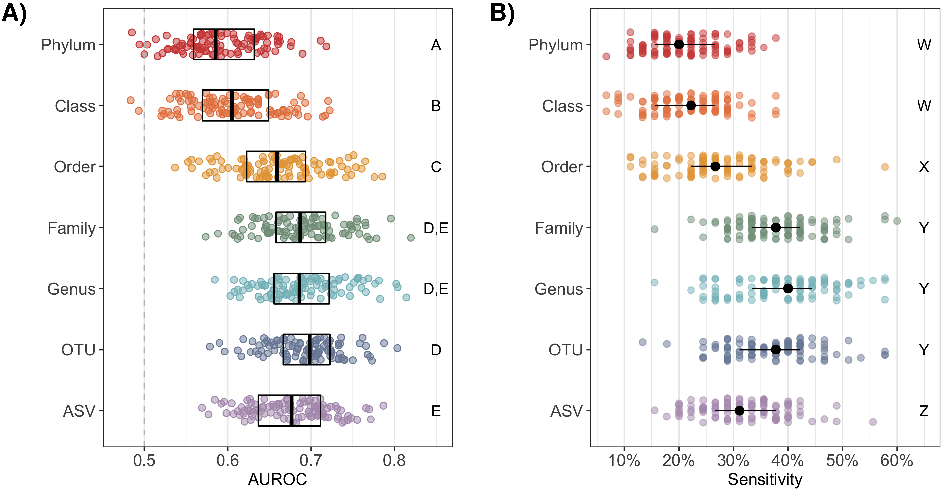
\includegraphics{manuscript_files/figure-latex/fig1-1.pdf}

\textbf{Figure 1: Random Forest Model Performance.} \textbf{A)} Boxplots
with points of area under the receiver operating characteristic curve
(AUROC) values on the test dataset for 100 seeds predicting SRNs using a
Random Forest model. Dashed line denotes AUROC of 0.5 which is
equivalent to random classification. Significance between taxonomic
levels was quantified by comparing the difference in mean AUROC and is
denoted by letters A through E on the right side of the plot; taxonomic
levels with the same letter are in the same significance group and are
not significantly different from one another. \textbf{B)} Strip plot of
the sensitivity at a specificity of 90\% across the 100 model
iterations. Black points denote the median and the lines denote the IQR.
The letters W through Z denote the significance groups.

\newpage

\hypertarget{tables}{%
\subsection{Tables}\label{tables}}

\begin{longtable}[]{@{}lrrc@{}}
\toprule
Taxonomic Level & Number of Features &
\makecell[c]{Number of Features \\ After Preprocessing} &
\makecell[c]{Percent of Features Kept \\ After Preprocessing} \\ \addlinespace
\midrule
\endhead
Phylum & 19 & 9 & 47.4 \% \\ \addlinespace
Class & 36 & 19 & 52.8 \% \\ \addlinespace
Order & 65 & 28 & 43.1 \% \\ \addlinespace
Family & 124 & 54 & 43.5 \% \\ \addlinespace
Genus & 316 & 115 & 36.4 \% \\ \addlinespace
OTU & 20079 & 705 & 3.5 \% \\ \addlinespace
ASV & 104106 & 478 & 0.5 \% \\ \addlinespace
\bottomrule
\end{longtable}

\textbf{Table 1: Summary of Features.} Overview of the number of
features at each taxonomic level before and after preprocessing as
described in the methods.

\newpage

\hypertarget{supplemental-figures}{%
\subsection{Supplemental Figures}\label{supplemental-figures}}

\includegraphics{../exploratory/figures/all_model_level.png}

\textbf{Supplemental Figure 1: Model Performance across Taxonomy.}
Boxplot of AUROC values on the test dataset for 100 seeds for each model
type across all taxonomic levels.

\newpage

\includegraphics[width=\textwidth,height=0.5\textheight]{../exploratory/figures/roc_by_level.png}

\textbf{Supplemental Figure 2: Averaged ROC curves} ROC curves averaged
across the 100 iterations of the model. The shaded region represents the
standard deviation form the mean.

\newpage

\includegraphics[width=\textwidth,height=0.45\textheight]{../exploratory/figures/bin_prevalence.png}\\
\textbf{Supplemental Figure 3: Prevalence of Taxa in Samples.}
Distribution of taxa prevalence in samples at each taxonomic level.

\newpage

\includegraphics[width=\textwidth,height=0.85\textheight]{../exploratory/figures/top10_imp.png}\\
\textbf{Supplemental Figure 4: Top 10 important taxa at each taxonomic
level.} Summary of the 10 most important taxa for the random forest
models at each taxonomic level based on the average decrease in AUC when
the feature is permuted.

\newpage

\hypertarget{references}{%
\subsection*{References}\label{references}}
\addcontentsline{toc}{subsection}{References}

\hypertarget{refs}{}
\begin{CSLReferences}{0}{1}
\leavevmode\hypertarget{ref-siegel2020}{}%
\CSLLeftMargin{1. }
\CSLRightInline{\textbf{Siegel RL}, \textbf{Miller KD}, \textbf{Sauer
AG}, \textbf{Fedewa SA}, \textbf{Butterly LF}, \textbf{Anderson JC},
\textbf{Cercek A}, \textbf{Smith RA}, \textbf{Jemal A}. 2020. Colorectal
cancer statistics, 2020. CA: A Cancer Journal for Clinicians
\textbf{70}:145--164. doi:\url{https://doi.org/10.3322/caac.21601}.}

\leavevmode\hypertarget{ref-garcuxeda2011a}{}%
\CSLLeftMargin{2. }
\CSLRightInline{\textbf{García G}, \textbf{Z A}. 2011. Factors
Influencing Colorectal Cancer Screening Participation. Gastroenterology
Research and Practice \textbf{2012}:e483417.
doi:\href{https://doi.org/10.1155/2012/483417}{10.1155/2012/483417}.}

\leavevmode\hypertarget{ref-callahan2017}{}%
\CSLLeftMargin{3. }
\CSLRightInline{\textbf{Callahan BJ}, \textbf{McMurdie PJ},
\textbf{Holmes SP}. 2017. Exact sequence variants should replace
operational taxonomic units in marker-gene data analysis. The ISME
Journal \textbf{11}:2639--2643.
doi:\href{https://doi.org/10.1038/ismej.2017.119}{10.1038/ismej.2017.119}.}

\leavevmode\hypertarget{ref-topuxe7uolu2020}{}%
\CSLLeftMargin{4. }
\CSLRightInline{\textbf{Topçuoğlu BD}, \textbf{Lesniak NA},
\textbf{Ruffin MT}, \textbf{Wiens J}, \textbf{Schloss PD}. 2020. A
Framework for Effective Application of Machine Learning to
Microbiome-Based Classification Problems. mBio \textbf{11}.
doi:\href{https://doi.org/10.1128/mBio.00434-20}{10.1128/mBio.00434-20}.}

\leavevmode\hypertarget{ref-callahan2016}{}%
\CSLLeftMargin{5. }
\CSLRightInline{\textbf{Callahan BJ}, \textbf{McMurdie PJ},
\textbf{Rosen MJ}, \textbf{Han AW}, \textbf{Johnson AJA}, \textbf{Holmes
SP}. 2016. DADA2: High-resolution sample inference from Illumina
amplicon data. Nature Methods \textbf{13}:581--583.
doi:\href{https://doi.org/10.1038/nmeth.3869}{10.1038/nmeth.3869}.}

\leavevmode\hypertarget{ref-lobo2008}{}%
\CSLLeftMargin{6. }
\CSLRightInline{\textbf{Lobo JM}, \textbf{Jiménez-Valverde A},
\textbf{Real R}. 2008. AUC: a misleading measure of the performance of
predictive distribution models. Global Ecology and Biogeography
\textbf{17}:145--151.
doi:\href{https://doi.org/10.1111/j.1466-8238.2007.00358.x}{10.1111/j.1466-8238.2007.00358.x}.}

\end{CSLReferences}

\end{document}
